\chapter{In-Context Learning}\label{chap:in-context-learning}

% There will be:
% \begin{itemize}
%     \item Definition of in-context learning (ICL),
%     \item References to studies supporting the usefulness of ICL for repository-level code completion capabilities of Code LLMs,
%     \item Discussion on prompt engineering,
%     \item Comparison of zero-shot, one-shot, and few-shot learning.
% \end{itemize}

% \chapter{Long Context}\label{chap:long-context}
% The following topics will be covered:
% \begin{itemize}
%     \item The significance of long context for in-context learning,
%     \item An overview of the challenges associated with long context, such as the quadratic dependency of computational resources on context length, the inability of RoPE to extrapolate, and the noise generated by softmax-based attention,
%     \item Strategies for addressing long context challenges, including memory-efficient attention implementations, key-value (KV) caching, gradient checkpointing, retrieval-augmented generation (RAG), subquadratic attention, and context extension methods.
% \end{itemize}

% TODO: chapter definition

\section{Definition}

In-context learning (ICL) refers to the ability of a model to condition on a set of demonstrations provided in the input context in order to learn and adapt to unseen tasks without modifying the parameters \parencite{brown2020}. The input string is called a \textit{prompt}, and typically includes a task description along with a set of examples. This paradigm of learning has proven highly effective, as it enables specialized approaches to solving tasks based solely on inference computations, while the model is pre-trained without awareness of task specificity.

\section{Long Context}

ICL introduces context length as a new scaling direction for LLMs \parencite{kaplan2020}. The terminology also encompasses the concepts of \textit{zero-shot}, \textit{one-shot}, and \textit{few-shot prompting}, which refer to the number of demonstrations provided in the prompt. Increasing the number of demonstrations typically leads to improved downstream performance \parencite{brown2020}.

However, leveraging the advancements of this scaling direction requires addressing multiple challenges. The following overview develops a fundamental understanding of some of the problems associated with long context in this field.

\subsection{Quadratic Complexity}  % TODO: better name

The original attention architecture of Transformer models exhibits quadratic computational and time complexity requirements, which depend on the number of tokens provided to the model \parencite{vaswani2017}. This undesirable property has prompted the development of numerous subquadratic and other efficient attention mechanisms. For instance, the survey by \citet{tay2022} offers a detailed examination of this subject and visualizes the taxonomy of such architectures, as shown in Figure~\ref{fig:taxonomy-of-transformers}.

\begin{figure}[ht]
    \centering
    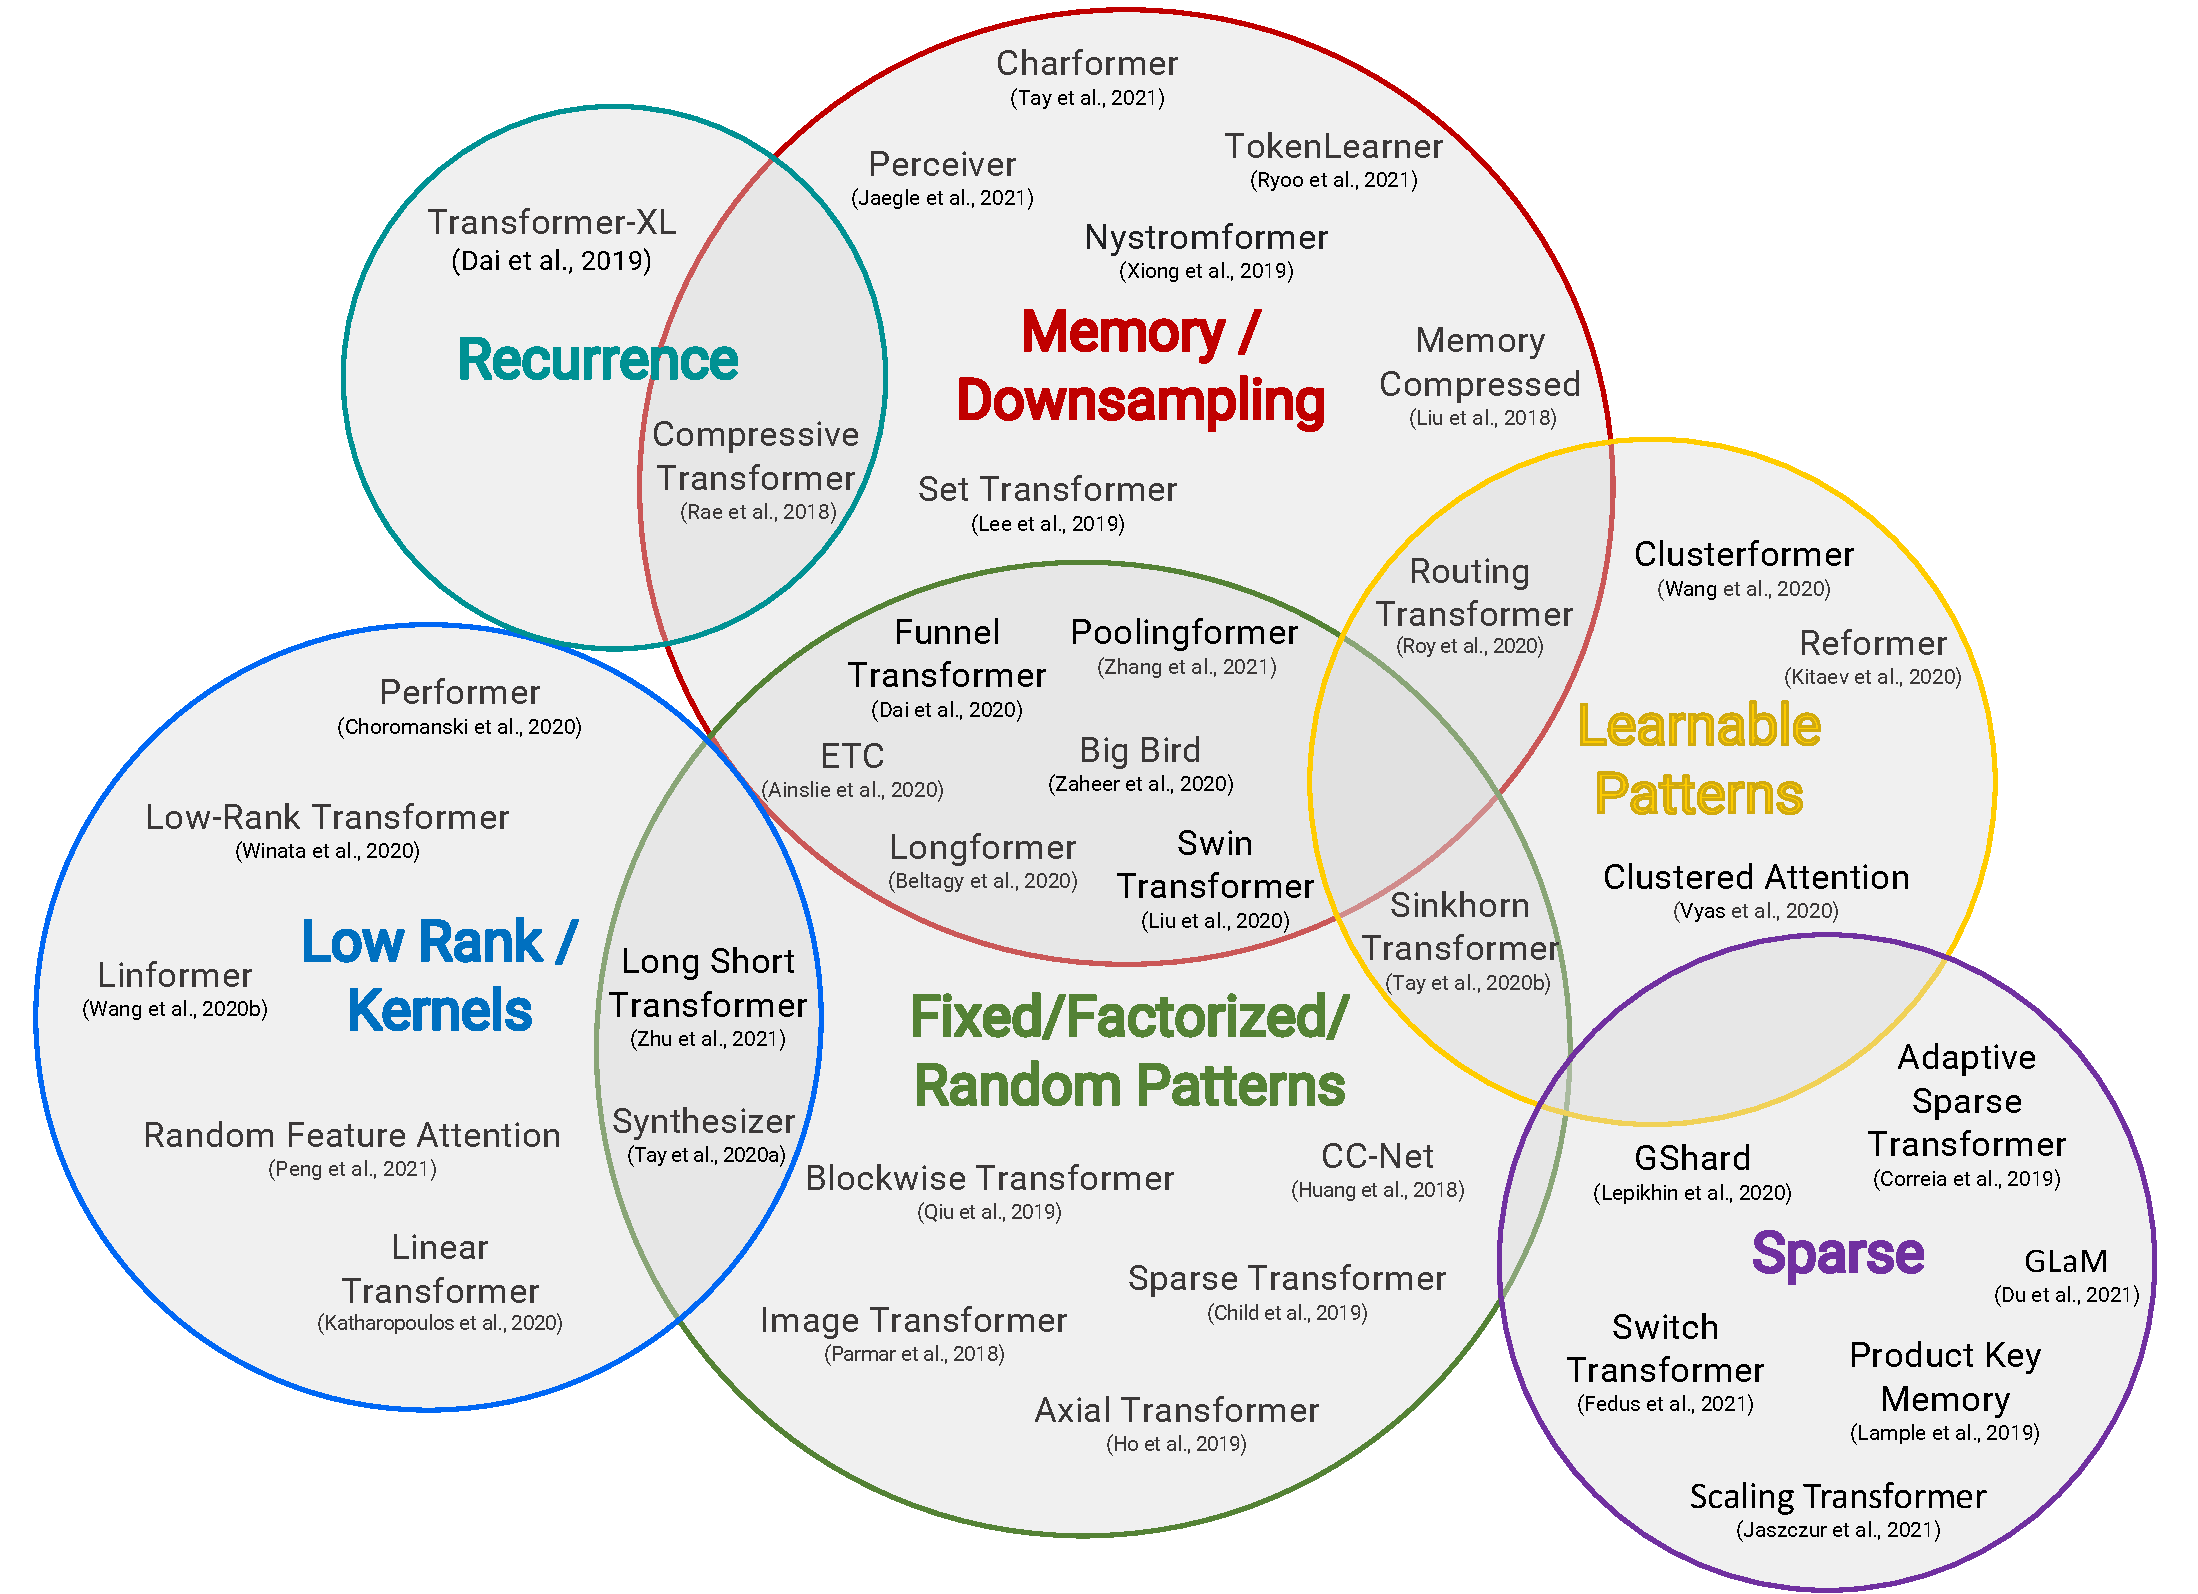
\includegraphics[width=\textwidth]{figures/taxonomy-of-transformers.pdf}
    \caption{Taxonomy of Efficient Transformer Architectures}\label{fig:taxonomy-of-transformers}
    \hfill\textit{Source: \citet{tay2022}}
\end{figure}



\subsection{Retrieval-Augmented Generation}
% TODO: prompt engineering

% TODO: ABF

\section{Code Completion}  % TODO: better name

ICL emerges during the training of large language models via the next-token prediction objective as a function of the number of parameters and the data size used for pre-training \parencite{hahn2023}. Thus, its presence is found in base models, which are used to perform the code completion task.
